\documentclass{article}
\usepackage[utf8]{inputenc}
\usepackage{amsmath}
\usepackage{mathtools}
\usepackage{hyperref}
\usepackage{graphicx}
\usepackage{verbatimbox}
\usepackage{float}
\usepackage{hyperref}
\usepackage[most]{tcolorbox}


\title{\bf{Gu\'ia pr\'actica de Root}}
\author{Sergio Best}
\date{\it{2016}}
\begin{document}
    \begin{figure}
    \begin{center}
    
\includegraphics[scale=0.25]{logo.png}
    \end{center}
    \end{figure}
\maketitle

Root es un entorno de an\'alisis de datos ampliamente utilizado en f\'isica de altas energ\'ias. Es la base de muchos simuladores usado en experimentos de colisionadores como Aliroot para ALICE en el LHC. Esta gu\'ia tiene como objetivo dar un primer vistazo de forma r\'apida y pr\'actica a las herramientas disponibles en Root. \par
Instalar Root en Linux \footnote{Se recomienda usar Root en un sistema operativo con Linux. Si quieres conservar tu Windows, hay formas de hacer Dual Boot con ambos sistemas. \url{https://help.ubuntu.com/community/WindowsDualBoot}} es bastante sencillo con solo las librer\'ias b\'asicas. Basta con descargar el source distribution de esta p\'agina: \url{https://root.cern.ch/downloading-root} y ejecutar el make. Para el momento de escribir esta gu\'ia la versi\'on estable era la 5.34. Si la \'ultima versi\'on es relativamente nueva, es mejor usar la anterior. Este es el caso para muchas distribuciones en Linux, incluyendo sistemas operativos. Usar una versi\'on m\'as antigua asegura que ya no hay tantos bugs, adem\'as de que hay m\'as ayuda disponible en los foros.
\begin{center}
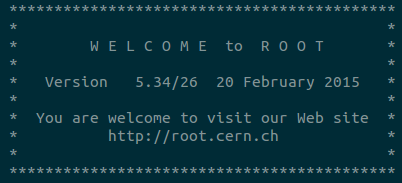
\includegraphics[scale=0.65]{welcome.png}
\end{center}
Una vez instalado correctamente basta con ejecutar Root desde terminal escribiendo root. \footnote{Si no funciona, lo m\'as probable es que las variables de entorno est\'en mal puestas. Esto se resuelve al ejecutar el archivo thisroot.sh que est\'a en la carpeta donde instalaste Root. Si no funciona puedes revisar las variables de entorno. Deben estar conectadas correctamente ROOTSYS, PATH y LD\_LIBRARY\_PATH. Puedes revisar a qu\'e est\'an conectadas escribiendo en terminal, por ejemplo: echo \$PATH}. 
Algunas de las opciones m\'as \'utiles a la hora de llamar a root en terminal son por ejemplo -l (para saltear la presentaci\'on), -b (para que no se abran los plots al ir ejecutando) y -q (para que se cierre root al terminar de ejecutar). \footnote{La opci\'on de -q es especialmente \'util cuando se est\'a ejecutando Root dentro de una macro de bash.} \par
Ejemplo:

\begin{tcolorbox} [breakable]
\begin{verbatim}
user@system: root -l
\end{verbatim}
\end{tcolorbox}

Si tu Root ya est\'a funcionando, entonces podemos empezar con esta gu\'ia. Hay tres secciones \footnote{El nombre de los niveles es solo referencial ya que todo lo presentado es b\'asico en Root y por tanto bastante usado.} con ejemplo y un ejercicio al final de cada una. Los c\'odigos se presentan en cajas grises y pueden copiarse, pero todos est\'an en el Git\footnote{\url{www.sergio.com}} de donde se pueden descargar directamente. \footnote{El c\'odigo en \LaTeX de este documento tambi\'en est\'a disponible en el Git.}
\newpage
\section{Nivel b\'asico}
\subsection{Operaciones matem\'aticas}
Ejecutando Root desde terminal, este se puede utilizar como una calculadora. Se pueden usar todas las operaciones b\'asicas como en cualquier otro lenguaje de programaci\'on. \footnote{Root en el fondo es C++, aunque tambi\'en se puede utilizar PyRoot el cual trabaja con Python. Para esta gu\'ia se usar\'a exclusivamente Root con C++.}
\begin{tcolorbox} [breakable]
\begin{verbatim}
root [0] 23+19
(const int)42
root [1] 6*7
(const int)42
\end{verbatim}
\end{tcolorbox}
Aqu\'i Root asume los valores como integers y da la respuesta tambi\'en como integer. Esto no es problema usualmente a menos que estemos haciendo una divisi\'on. Para este caso colocamos el n\'umero con punto decimal, aunque no pongamos ning\'un decimal despu\'es.
\begin{tcolorbox} [breakable]
\begin{verbatim}
root [2] 7/2
(const int)3
root [3] 7./2
(const float)3.5
\end{verbatim}
\end{tcolorbox}
Tambi\'en podemos usar funciones cl\'asicas. En este ejemplo usamos coseno, exponencial y arcocoseno.
\begin{tcolorbox} [breakable]
\begin{verbatim}
root [4] cos(TMath::Pi())
(const double)-1.00000000000000000e+00
root [5] exp(3.)
(const double)2.00855369231876679e+01
root [6] acos(-1.)
(const double)3.14159265358979312e+00
\end{verbatim}
\end{tcolorbox}
Hay una lista completa de funciones disponibles en \url{https://root.cern.ch/root/html524/TMath.html}
\subsection{Histogramas}

Los histogramas en root son de la forma TH(1-2)X.
Donde el n\'umero puede ser 1 ó 2 dependiendo de la dimensi\'on del histograma y X es el tipo de variable que acepta el histograma. X puede ser F (float), I (integer), D (double).\newline
Por ejemplo TH1F, es un histograma de una dimension que acepta floats.
Lo definimos:
\begin{tcolorbox} [breakable]
\begin{verbatim}
//Este histograma abarca el rango de -10 a 10,
//divididos en 1000 intervalos.
TH1F* hist=new TH1F("Name","Title",1000,-1.,1.)
//Y lo llenamos con
hist -> Fill(0.314159)
\end{verbatim}
\end{tcolorbox}
Al llenar el histograma, Root bota un n\'umero. Este n\'umero es el intervalo en el que cae el valor introducido (el 0.314159). Un histograma solo asocia un n\'umero (en este caso el n\'umero de veces que un valor cay\'o en el intervalo), as\' que ocupa menos espacio, pero se pierde la informaci\'on de exactamente qu\'e n\'umeros entraron.
\footnote{Tambi\'en se puede escribir sin punteros y en este caso se usar\'ia un punto (.) en lugar de (-$>$). En esta gu\'ia se usar\'an punteros en la mayor\'ia, si no es en todos los casos.}
\subsection{Macros}

Ahora, el potencial de Root no est\'a en la l\'inea de comando, sino en utilizar macros. Estas se escriben igual que una macro en C++, pero se pueden usar objetos definidos para root, tales como los histogramas que vimos o Trees para guardar información. Estas macros despu\'es se ejecutan en terminal de la siguiente forma: \newline

\begin{tcolorbox} [breakable]
\begin{verbatim}
user@system: root -l 'macro.C'
\end{verbatim}
\end{tcolorbox}

A partir de ahora dar\'e el c\'odigo listo para ejecutar:

\begin{tcolorbox} [breakable]
\begin{verbatim}
#include "TH1F.h"
#include "TH2F.h"
#include "TMath.h"
#include <stdio.h>
#include <fstream>

Int_t Example1 () {
  TH1F * hist = new TH1F ("hist","Title",100,0.,50.);
  //¡Ahora si no olvides los punto y comas!
  for (Int_t i;i<100;i++ ){
     //Como pasado i=50 caen fuera del rango
     //entonces no entran en el histograma.
     hist->Fill(i);
  }
  return 1;
}
\end{verbatim}
\end{tcolorbox}

\subsection{Dibujando}

Para empezar a dibujar usamos un lienzo. Para Root esto es el TCanvas.
\begin{tcolorbox} [breakable]
\begin{verbatim}
//Empezamos con el mismo codigo que antes
#include "TH1F.h"
#include "TH2F.h"
#include "TCanvas.h"

Int_t Example2 () {
  TH1F * hist = new TH1F ("hist","Title",100,0.,50.);
  //¡Ahora si no olvides los punto y comas!
  for (Int_t i=0;i<100;i++ ){
     //Como pasado i=50 caen fuera del rango
     //entonces no entran en el histograma.
     hist->Fill(i);
  }
  
Float_t ancho = 600;
Float_t alto = 400;

TCanvas * c1 = new TCanvas();
//Root dibuja sobre el canvas activo.
//En este caso es el unico que hemos definido.
c1->SetCanvasSize(ancho,alto);
hist->Draw();
TCanvas * c2 = new TCanvas();
c2->SetCanvasSize(ancho,alto);
//Solo podemos tener un canvas activo.
//Cuando se define un nuevo canvas, ese es el activo.
//Pero podemos cambiar de canvas usando:
c1->cd();

//Tambien podemos dividir el canvas en pads.
Int_t nColumnas = 3;
Int_t nFilas = 2;
c2->Divide(nColumnas,nFilas);
//Y cambiamos el subcanvas activo con:
c2->cd(1);
hist->Draw();
c2->cd(3);
hist->Draw();
c2->cd(5);
hist->Draw();
//Por cierto, aunque solo uno de los subcanvas este activo, 
//al usar Draw se dibujaran todos los subcanvas juntos.

  return 1;
}
\end{verbatim}
\end{tcolorbox}

\subsection{Grabando plots}

Dentro del c\'odigo, se puede grabar el plot usando la funcion: \newline
\begin{tcolorbox} [breakable]
\begin{verbatim}
c1->SaveAs("./imagen.png");
\end{verbatim}
\end{tcolorbox}
El par\'ametro es la direcci\'on donde se guarda la imagen adem\'as del nombre de la imagen y su formato. Formato recomendado: PNG. './' significa que es en el directorio actual, es decir directorio donde se abri\'o root. \par
Se puede grabar desde el canvas que se abre al ejecutar el codigo yendo a File$>$Save...

\begin{center}
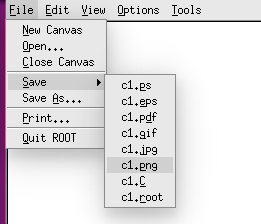
\includegraphics[scale=0.65]{save.png}
\end{center}

Por cierto, si se ha usado la opcion -b al ejecutar root, la imagen se graba del tamaño establecido del canvas. Por eso es importante definir el tamaño del canvas usando SetCanvasSize. Si no tienes suficiente resoluci\'on, por ejemplo porque has dividido el canvas en varios pads, entonces ya no se podr\'a leer bien.


\subsection{Juntando todo}
\par
Ahora que sabemos c\'omo hacer las cosas b\'asicas, podemos pasar a ver un c\'odigo completo. En este archivo tenemos pares de electr\'on-positr\'on, algunos podr\'ian venir del decaimiento de un J/$\psi$, asi que calculamos la masa de la part\'icula original y buscamos un pico.

\begin{tcolorbox} [breakable]
\begin{verbatim}

#include "TH1F.h"
#include "TH2F.h"
#include "TF1.h"
#include "TMath.h"
#include "TGraph.h"
#include "TString.h"
#include "TCanvas.h"
#include <stdio.h>
#include <fstream>
//Librerias utiles para lo que haremos.

Int_t jpsi() {
//El nombre y direccion del archivo de donde leemos los datos
TString fName = "./jpsi.dat";
//Abrimos la comunicacion con el archivos
ifstream rawfile(fName.Data());
//En caso el programa no encuentre el archivo, dara este error. 
//Si no esta esto la terminal se cuelga.
if(!rawfile.good()) {
        cout << "File not found!" << endl;
        return 0;
}

//Definimos variables para leer los datos.
Int_t Run;
Double_t Event;
Float_t E1;
Float_t E2;
Float_t PX1;
Float_t PZ1;
Float_t PT1;
Float_t PX2;
Float_t PZ2;
Float_t PT2;

TH1F *jpsi =
new TH1F("jpsi","J/Psi;Mass[GeV/c2];Counts",250,2.,5.)
//El punto y coma en el titulo es una forma
//rapida de poner titulos a los ejes.
while(rawfile >> Run>>Event>>E1>>PX1>>PY1>>PZ1
>>PT1>> E2>>PX2>>PY2>>PZ2>>PT2 && rawfile.good()){
        //La funcion pow es 'elevado a la...'
	Float_t mass = pow((pow((E1+E2),2)-pow((PX1+PX2),2) 
	-pow((PY1+PY2),2)-pow((PZ1+PZ2),2)),0.5);
	jpsi->Fill(mass);
}

TCanvas * c1 = new TCanvas();
c1->SetCanvasSize(1200,700);
jpsi->SetLineWidth(2.5);
jpsi->SetLineColor(kRed);
jpsi->SaveAs("./JPSI.sh")
c1->Draw();

return 1;
}
\end{verbatim}
\end{tcolorbox}

No funcion\'o, ¿cierto? Para completar el cap\'itulo debes encontrar que est\'a mal con el c\'odigo. \newline
Puedes guiarte de los errores que da el compilador. Revisa que todo est\'e bien definido. Que se llamen a los objetos correctos. \par
\vspace{1cm}
\textbf{¡Buena suerte! Nos vemos en el pr\'oximo cap\'itulo.}

\newpage
\section{Nivel Intermedio}

\subsection{Dominando los histogramas}

A veces llenar el histograma puede tomar mucho tiempo, especialmente si ya sabes cu\'anto debe ir en cada intervalo. Root nos permite cambiar los valores dentro del histograma, as\'i como tambi\'en de los errores.

\begin{tcolorbox} [breakable]
\begin{verbatim}
#include "TH1F.h"
#include "TH2F.h"
#include "TF1.h"
#include "TMath.h"
#include "TCanvas.h"
#include <stdio.h>
#include <fstream>
#include "TStyle.h"

Int_t Example3()
{
TH1F * hist = new TH1F("hist","Ejemplo",5,0.,5.);
//Aqui hay algo muy raro. Los intervalos se empiezan a contar
//desde el 1, no desde 0. El 0 y el N+1 estan reservados para
//valores por debajo o por encima del rango, respectivamente.
hist->SetBinContent(1,100.);
hist->SetBinContent(2,50.);
hist->SetBinContent(3,25.);
hist->SetBinContent(4,10.);
hist->SetBinContent(5,5.);
//Esta opcion es para dibujar con errores.
hist->Draw("E1");
return 1;
}
\end{verbatim}
\end{tcolorbox}
¿No es raro? ¿De d\'onde salieron los errores? El histograma solo cuenta cuantos valores caen dentro y olvida el resto. Es m\'as, ahora hemos colocado el valor directamente.
Como no hay un error asociado simplemente pone el error como la ra\'iz del valor. S\'e que suena arbitrario, pero es un procedimiento bastante com\'un dadas las distribuciones que se suelen ver.\par
Es bueno tener esto en cuenta, porque cuando hagamos ajustes, si los valores son muy pequeños (menores que 1), el error sale m\'as grande que el punto. Cualquier funci\'on pasa por ah\'i, as\'i que el ajuste saldr\'a mal.\\
Vamos a ver ahora c\'omo colocar los errores.
\begin{tcolorbox} [breakable]
\begin{verbatim}
#include "TH1F.h"
#include "TH2F.h"
#include "TF1.h"
#include "TMath.h"
#include <stdio.h>
#include <fstream>
#include "TStyle.h"

Int_t Example4()
{
Float_t x [5]= {100.,50.,25.,10.,50.};
Float_t errorx [5] = {1.,2.,3.,2.,1.};
TH1F * hist = new TH1F("hist","Ejemplo",5,0.,5.);
for (Int_t i = 1; i<=5;i++){
hist->SetBinContent(i,x[i-1]);
hist->SetBinError(i,errorx[i-1]);
}
hist->Draw("E");
//Y luego podemos recuperar un valor.
Float_t value = hist->GetBinContent(3);
cout<<"El valor del intervalo 3 es: "<< value<<endl;
return 1;
}
\end{verbatim}
\end{tcolorbox}

\subsection{Gr\'aficos}

Cuando se quieren presentar muchos sets de datos en un mismo plot, es m\'as ordenado presentarlos como Graphs. Empezaremos con el objeto m\'as sencillo de este tipo y llegaremos a gr\'aficos del estilo que se presentan en p\'articulas. \footnote{Aunque estos objetos piden arrays para trabajar, se puede usar vector (que usualmente se pueden trabajar mejor). Para usar vectores en un Graph, no pasamos todo el vector, sino solo el primer espacio de memoria. Eg:\newline
Graph * grafico = new Graph(x.length(),\&x[0],\&y[0]);
}

\subsubsection{Graph}

Un Graph es un gr\'afico simple, solo pone las coordenadas que se le dan como puntos.
\begin{align*}
x=&\begin{pmatrix}
         x_0 & x_1 & x_2 & x_3 & x_4
  \end{pmatrix}&\\
&\hskip 0.8em \downarrow \hskip 1.4em \downarrow \hskip 1.4em \downarrow \hskip 1.4em \downarrow  \hskip 1.4em \downarrow\\
y=&\begin{pmatrix}
       y_0 & y_1 & y_2 & y_3 & y_4
\end{pmatrix}
\end{align*}
Y forman los pares de coordenadas: \newline

$\begin{pmatrix}
       x_0 & y_0
\end{pmatrix} $\hskip 1.5em
$\begin{pmatrix}
       x_1 & y_1
\end{pmatrix}$ \hskip 1.5em
$\begin{pmatrix}
       x_2 & y_2
\end{pmatrix}$ \hskip 1.5em
$\begin{pmatrix}
       x_3 & y_3
\end{pmatrix}$ \hskip 1.5em
$\begin{pmatrix}
       x_4 & y_4
\end{pmatrix}$ \hskip 1.5em \newline

\begin{tcolorbox} [breakable]
\begin{verbatim}
#include "TH1F.h"
#include "TH2F.h"
#include "TF1.h"
#include "TMath.h"
#include "TGraph.h"
#include "TCanvas.h"
#include <stdio.h>
#include <fstream>

Int_t Example5()
{
Float_t x[5]={1.,2.,3.,4.,5.};
Float_t y[5]={5.,4.,3.,2.,1.};
//Entra el numero de elementos, y los dos vectores.
TGraph * grafico = new TGraph (5,x,y);
//Esta parte es solo estetica. El color y forma de los puntos.
grafico->SetMarkerColor(kRed);
grafico->SetMarkerStyle(kFullCircle);
//Y dibujamos el grafico.
TCanvas * c1 = new TCanvas();
\end{verbatim}
grafico-$>$Draw("APL");\footnote{Las opciones son: A para dibujar los ejes, si se dibujan varios Graphs en un mismo canvas, solo se pone esta opci\'on en el primero que se dibuja. P es para dibujar los puntos, L es para dibujar l\'ineas entre los puntos. El orden de las letras no importa.}
\end{tcolorbox}

\subsubsection{GraphErrors}

Aqu\'i usamos 4 arreglos en lugar de 2, esto es para sacar los errores correspondientes a cada punto en cada eje.

\begin{tcolorbox} [breakable]
\begin{verbatim}
#include "TH1F.h"
#include "TH2F.h"
#include "TF1.h"
#include "TMath.h"
#include "TGraph.h"
#include "TGraphErrors.h"
#include "TString.h"
#include "TCanvas.h"
#include <stdio.h>
#include <fstream>

Int_t Example6()
{
Float_t x[5]={1.,2.,3.,4.,5.};
Float_t y[5]={1.,4.,3.,2.,1.};
Float_t errorx[5]={0.1,0.2,0.3,0.4,0.5};
Float_t errory[5]={0.5,0.4,0.3,0.2,0.1};
TGraphErrors* grafico = new TGraphErrors (5,x,y,errorx,errory);
grafico->SetMarkerColor(kRed);
grafico->SetMarkerStyle(kFullCircle);
grafico->SetLineStyle(9);
grafico->SetLineColor(kBlue);
TCanvas* c1 = new TCanvas();
grafico->Draw("APL");
return 1;
}
\end{verbatim}
\end{tcolorbox}
Notar que al aplicar el estilo de la l\'inea, tambi\'en cambia el estilo de las barras de error, porque este es el mismo objeto. Un truco para resolver esto es agregar un segundo gr\'afico, sin estilo de l\'inea y dibujarlo encima sin la opci\'on de dibujo L. \newline 
\subsubsection{MultiGraph}
Para ver esto, usaremos un objeto que reune varios Graphs para dibujarlos todos juntos.
\begin{tcolorbox} [breakable]
\begin{verbatim}
#include "TH1F.h"
#include "TH2F.h"
#include "TF1.h"
#include "TFile.h"
#include "TTree.h"
#include "TMath.h"
#include "TGraph.h"
#include "TGraphErrors.h"
#include "TMultiGraph.h"
#include "TString.h"
#include "TCanvas.h"
#include <stdio.h>
#include <fstream>
#include "TStyle.h"
#include "TASImage.h"

Int_t Example7()
{
Float_t x[5]={1.,2.,3.,4.,5.};
Float_t y[5]={5.,4.,3.,2.,1.};
Float_t errorx[5]={0.1,0.2,0.3,0.4,0.5};
Float_t errory[5]={0.5,0.4,0.3,0.2,0.1};
TMultiGraph *multi = new TMultiGraph();
TGraphErrors *grafico=new TGraphErrors(5,x,y,errorx,errory);
TGraphErrors *grafico2=new TGraphErrors(5,x,y,errorx,errory);
multi->Add(grafico,"LP");
multi->Add(grafico2,"P");
grafico->SetMarkerColor(kRed);
grafico->SetMarkerStyle(kFullCircle);
grafico->SetLineStyle(9);
grafico->SetLineColor(kBlue);
grafico2->SetMarkerColor(kRed);
grafico2->SetMarkerStyle(kFullCircle);
multi->Draw("A");
return 1;
}
\end{verbatim}
\end{tcolorbox}

Ahora veremos la verdadera utilidad de MultiGraph.

\begin{tcolorbox} [breakable]
\begin{verbatim}
#include <string>
#include <vector>
#include <TCanvas.h>
#include <Riostream.h>
#include <TGraph.h>
#include <TGraphErrors.h>
#include <TMultiGraph.h>
#include <TString.h>
#include <TLegend.h>
#include <TH2F.h>
#include <TH1F.h>
#include <math.h>

//Datos extraidos del experimento AMS

Int_t Elements (){
Float_t electrons [74];
Float_t electronsFlux[74];
Float_t protons[72];
Float_t protonsFlux[72];
Float_t EMIN, EMAX, EMEAN,Y, STATMIN, STATMAX, SYSMIN ,SYSMAX;
Int_t count=0;

  FILE *fpElectrons = fopen("./electrons.txt", "r");
  while (fscanf (fpElectrons,"%f %f %f %f %f %f %f %f ", 
  &EMIN,&EMAX,&EMEAN,&Y,&STATMIN,&STATMAX,&SYSMIN,&SYSMAX)==8) 
  {
			electrons[count]=EMEAN;
			electronsFlux[count]=Y;
			count++;
			cout<<EMEAN<<endl;
  }
  fclose(fpElectrons);
  count = 0;
  FILE *fpProtons = fopen("./protons.txt", "r");
  while (fscanf (fpElectrons,"%f %f %f %f %f %f %f %f ", 
  &EMIN,&EMAX,&EMEAN,&Y,&STATMIN,&STATMAX,&SYSMIN,&SYSMAX)==8) 
  {
			protons[count]=EMEAN;
			protonsFlux[count]=Y;
			count++;
  }
  fclose(fpProtons);

  TMultiGraph *mg=new TMultiGraph();
  TCanvas *CanvasGraph = new TCanvas();

  TGraph* graficoElectrons=new TGraph(74,electrons,
  electronsFlux);
  graficoElectrons->SetMarkerStyle(21);
  graficoElectrons->SetMarkerColor(1);
  graficoElectrons->SetMarkerStyle(21);
  graficoElectrons->SetLineColor(kBlack);
  graficoElectrons->SetLineWidth(2);
  mg->Add(graficoElectrons,"P");

  TGraph* graficoProtons=new TGraph(72,protons,protonsFlux);
  graficoProtons->SetMarkerStyle(21);
  graficoProtons->SetMarkerColor(6);
  graficoProtons->SetMarkerStyle(21);
  graficoProtons->SetLineColor(kBlack);
  graficoProtons->SetLineWidth(2);
  mg->Add(graficoProtons,"P");

mg->SetTitle("Flux vs Energies");
gPad->Modified();
mg->Draw("A");
mg->GetXaxis()->SetTitle("Energia Cinetica[GeV]");
mg->GetYaxis()->SetTitle("Flujo[m^{-2}sr^{-1}s^{-1}GeV^{-1}]");

  TLegend *leg = new TLegend(0.65,0.6,0.9,0.9);
  leg->AddEntry(graficoElectrons,"e^{-} e^{+}: AMS-02", "p");
  leg->AddEntry(graficoProtons,"Protons: AMS-02", "p");
  leg->Draw();

  CanvasGraph-> SaveAs("./Graph.png");
return 1;
}
\end{verbatim}
\end{tcolorbox}

Veremos en el siguiente ejemplo c\'omo mejorar este plot con escala logar\'itmica.

\subsection{Ejes}

\subsubsection{Escala logar\'itmica}

Lo curioso de la escala logar\'itmica, y lo que hay que tener en cuenta, es que no se aplica sobre un eje o un histograma, sino que se aplica sobre el canvas. As\'i es, la escala logar\'itmica est\'a en el todo el canvas. De esta forma Root se asegura de que todos los objetos dibujados encima de este tengan la misma escala.\\
Agr\'egale estas dos l\'ineas de c\'odigo al ejemplo anterior para cambiarlo a escala logar\'itmica. Nota que los puntos ahora se pueden distinguir mejor, esta es la utilidad de la escala logar\'itmica y se usa casi siempre en los plots de part\'iculas.

\begin{tcolorbox} [breakable]
\begin{verbatim}
CanvasGraph->SetLogy();
CanvasGraph->SetLogx();
\end{verbatim}
\end{tcolorbox}

\subsubsection{L\'imites de los ejes}

Esto deber\'ia ser sencillo. Pero veamos las muchas opciones que hay para fijar l\'imites y cual nos conviene dependiendo del objeto con el que trabajemos.

Para Graphs:

\begin{tcolorbox} [breakable]
\begin{verbatim}
//En eje x
graph->GetXaxis->SetLimits(0.,100.);
//Pero para el eje Y
graph->SetMaximum(100.);
graph->SetMinimum(0.);
//Tambien podemos usar SetRange, esto es mejor
//porque se usa el mismo para todos los ejes.
graph->GetXaxis->SetRangeUser(0.,100.);
graph->GetYaxis->SetRangeUser(50.,500.);
\end{verbatim}
\end{tcolorbox}

Para histogramas:

\begin{tcolorbox} [breakable]
\begin{verbatim}
hist->GetXaxis->SetLimits(0.,100.);
hist->GetYaxis->SetLimits(-100.,50.);
\end{verbatim}
\end{tcolorbox}

Pru\'ebalo para los c\'odigos de arriba.

\subsection{N\'umeros aleatorios}

Tenemos en Root los objetos TRandom que son generadores de n\'umeros aleatorios. Hay principalmente dos factores a tomar en cuenta al elegir un generador de n\'umeros aleatorios. El tiempo que se demora en generar un n\'umero aleatorio (usualmente en el orden de nanosegundos, pero recuerda que usualmente se generan millones de estos). Otro factor a tener en cuenta es el periodo en que se repiten los n\'umeros. El generador recibe una semilla que es un n\'umero, calcula un n\'umero aleatorio y cambia sus condiciones para generar el siguiente, cuando se repiten las condiciones iniciales entonces los siguientes n\'umeros que genere ser\'an los mismos del principio. Esto es malo porque estos ya no se ven como n\'umeros aleatorios sino como repetidos.

\begin{tcolorbox} [breakable]
\begin{verbatim}
#include "TH1F.h"
#include "TH2F.h"
#include "TF1.h"
#include "TMath.h"
#include "TGraph.h"
#include "TString.h"
#include "TCanvas.h"
#include <stdio.h>
#include <TRandom3.h>
#include <fstream>

Int_t Example8()
{
TRandom * generadorX = new TRandom3();
//Podemos definir mas de un generador de numeros aleatorios.
//Esto es para probar la aletoriedad de nuestro generador.
//Puedes elegir otros generadores para compararlos.
TRandom * generadorY = new TRandom3();
TH2F * hist = new TH2F ("hist","Titulo",1000,0.,1.,1000,0.,1.);
Float_t x;
Float_t y;
//Hacemos avanzar el generador un paso.
x=generadorX->Rndm();
for (Int_t i = 0;i<3000000;i++){
//Vemos correlacion entre randoms consecutivos.
//Puedes probar con ->Gaus() para ver sesgo
	x = generadorX->Rndm();
	y = generadorY->Rndm();
	hist->Fill(x,y);
}
//Esto dibuja el eje Z con colores.
hist->Draw("COLZ");
return 1;

}
\end{verbatim}
\end{tcolorbox}

Puedes probar con los otros generadores. TRandom, TRandom1, TRandom2, TRandom3. Sus especificaciones est\'an en: \url{https://root.cern.ch/doc/master/classTRandom.html}

\subsection{Fits y Funciones}

Para hacer un ajuste de datos primero aprenderemos como definir funciones en Root.

\begin{tcolorbox} [breakable]
\begin{verbatim}
#include "TH1F.h"
#include "TH2F.h"
#include "TF1.h"
#include "TRandom3.h"
#include "TMath.h"
#include "TGraph.h"
#include "TString.h"
#include "TCanvas.h"
#include <stdio.h>
#include <fstream>
#include "TStyle.h"
#include "TASImage.h"

Int_t Example9()
{
//Para hacer un fit definimos funciones con parametros libres.
TF1* f1 =new TF1("f1","[0]*x*x+sin(x*[1])",-5.,5.);
//Los numeros en corchetes son los parametros libres.
//Los podemos setear de la siguientes formas...
//Uno por uno:
f1->SetParameter(0,500.);
f1->SetParameter(1,350.);
//O todos de una sola vez:
f1->SetParameters(500.,350.);
//Cuando root intenta hacer el fit, busca desde este valor.
//Es mas rapido, encuentra mejor el punto que buscas.
\end{verbatim}
\end{tcolorbox}

Ahora creamos un set de datos para hacer el ajuste.
\begin{tcolorbox} [breakable]
\begin{verbatim}
TH1F * hist = new TH1F ("hist","Titulo",100,-3.,3.);
TRandom3 * r = new TRandom3();
Float_t x;
for (Int_t i = 0;i<10000;i++){
x=r->Gaus();
hist->Fill(x);
}
hist->Draw();
//La cual ajusta pesimamente.
hist->Fit("f1");
//Esta sale mejor. Porque de ahi sacamos los datos.
hist->Fit("gaus","+");
return 1;

}
\end{verbatim}
\end{tcolorbox}

\subsection{Juntando todo}

El pAlpide es un chip que se usa para detectar el paso de part\'iculas midiendo la carga que pasa por cada pixel individual de detecci\'on. Un test que podemos hacer para probar su sensibilidad es pasarle carga artificialmente. Del archivo, las dos primeras columnas son la direcci\'on del pixel, luego la carga inyectada, y la \'ultima es cuantas veces responde (de 50). As\'i que podemos graficar la curva de respuesta vs carga, ajustarla y obtener la media de la funci\'on como valor representativo.

\begin{tcolorbox} [breakable]
\begin{verbatim}
#include "TF1.h"
#include "TMath.h"
#include "TGraph.h"
#include "TString.h"
#include "TCanvas.h"
#include <stdio.h>
#include <fstream>
#include <iostream>
#include <math.h>
#include "TGaxis.h"
#include "TAxis.h"
#include <string>
using namespace std;

int chargeMax = 89;
int chargeMin = 0;
int nInj = 50;
int data[256]={0};
int x   [256]={0};
int NPoints;
char fNameOut [50];
char separacion= 95;
int ELECTRONS_PER_DAC = 7; 
int fila, columna;
int NPixels=0;
int NNostart;
int NChisq;

void ResetData() {
  for (int i=0; i <= 255; i++) 
  {
    data[i] = 0;
  }
}

Double_t erf( Double_t *xx, Double_t *par){
  return (nInj / 2) *TMath::Erf((xx[0] - par[0]) / 
  (sqrt(2) *par[1])) +(nInj / 2);
}

Float_t FindStart (int NPoints, int *xx, 
int *data,int col,int addr) {
  float Upper = (float)xx[NPoints-1];
  float Lower = (float)xx[0];
  int up = data[NPoints-1];
  int down = data[0];
  int reachUp = 1;
  int reachDown = 1;

  	for (int i = 2; i < NPoints+1; i ++) 
        {
        if(up==50){reachUp=0;}
        //Revisa por un flanco de bajada. 
        //Si lo encuentra se queda con el valor de la posicion.
		if (up > data[NPoints -i] ) 
		{Upper = (float) xx[NPoints-i]; break;}
		up = data[NPoints - i];
        }

  	for (int i = 1; i < NPoints ; i++) 
        {
        if(down==0){reachDown=0;}
        //Revisa por un flanco de subida. 
        Si lo encuentra se queda con el valor de la posicion.
		if (down < data[i] ) {Lower = (float) xx[i];break;}
		down = data[i];
	}
 
  	if ((Upper==(float)xx[NPoints-1])||
  	(Lower==(float)xx[0])){
        //Nunca hubo flanco de subida o bajada
		if(data[0]==50)
		{cout<<"Hot Pixel: "<< col <<" "<<addr<<endl;return -1; }
		if(data[0]==0)
		{cout<<"Dead Pixel: "<< col <<" "<<addr<<endl;return -1; }
	}

    if (reachUp)
    {std::cout<<"Not enough charge to activate pixel: "
    <<col <<" "<< addr <<std::endl;}
    if (reachDown)
    {std::cout<<"Too much charge to start with pixel: "
    <<col <<" "<< addr <<std::endl;}
    //Da una idea de donde podria estar el medio.
	return (Upper + Lower)/2;

}

bool GetThreshold(double *AThreshold, double *ANoise, 
double *AChisq, bool *Ascurve, int col, int addr) {

   TGraph * g = new TGraph (NPoints,x,data);
   TF1 *fitfcn = new TF1("fitfcn", erf,0,500,2);
   //Valor posiblemente cercano a la media.
   Float_t Start  = FindStart(NPoints, x, data, col, addr);
   if (Start == -1) { //Dead or Hot pixel
     NNostart ++;
     std::cout << "Pixel "<<col<<" "<< addr <<
     " has no start point. Assigning start point to the 
     middle."
     << std::endl;
     Start = (chargeMax+chargeMin)*ELECTRONS_PER_DAC/2.;
     *Ascurve = true;
   }
   else {*Ascurve = false;}

   fitfcn->SetParameters(Start,10);
   fitfcn->SetParName(0, "Threshold");
   fitfcn->SetParName(1, "Noise");
   g->Fit("fitfcn","Q");

   //Obteniendo los valores
   *ANoise     = fitfcn->GetParameter(1);
   *AThreshold = fitfcn->GetParameter(0);
   *AChisq     = fitfcn->GetChisquare()/fitfcn->GetNDF();
   g->Delete();
   fitfcn->Delete();
   if (*AThreshold>(ELECTRONS_PER_DAC*chargeMax) 
   || *AThreshold<0){*Ascurve = true;}
   return true;
}

Int_t ProcessPixel (int col, int addr, 
const char *fName, FILE * fpoutResults) {
  double Threshold = 0;
  double Noise = 0;
  double Chisq = 0;
  bool scurve = false;
  if ( ((col%10) == 0)&&((addr%1000 == 0)) ) {
  cout <<"We are in col: " <<col << " of 512" <<endl;}
  if (!GetThreshold (&Threshold, &Noise,
  &Chisq, &scurve ,col, addr))
  {
          cout<<"Couldn't get Threshold of Pixel: "
          <<col<<" "<<addr<<endl;
  }
  fprintf(fpoutResults, 
  "%d %d %.2f %.2f %.2f\n", col,addr,Threshold,Noise,Chisq);
  if (scurve) 
  //Se ha mandado a dibujar el scurve de este pixel.
  {
	     cout<<"Drawing S-Curve: "<<col<<"-"
	     << addr<<" with Threshold: "<<Threshold<<endl;
	     TString colName;
	     colName.Form("%d",col);
	     TString addrName;
	     addrName.Form("%d",addr);
	     TString thresholdName;
	     thresholdName.Form("%.2f",Threshold);
	     //Cuando vuelva a pasar por aqui, 
	     //se vuelve a hacer el canvas, no hay problema.
	     TCanvas *wrongPixel = new TCanvas();
         wrongPixel->cd();
	     TLine *thresholdLine;
	     TGraph* curve = new TGraph (NPoints, x, data);   
	     curve->SetMarkerStyle(21);
	     curve->GetXaxis()->SetTitle("Charge [e]");
	     curve->GetYaxis()->SetTitle("Nhits");
	     curve->SetMaximum(50);
         curve->SetMinimum(0);
	     TString Title="DoubleColumn: ";
	     Title = Title + colName+ " Address: 
	     "+addrName+" Threshold: "+ thresholdName;
	     curve->SetTitle(Title);
         //Dibujar la funcion de ajuste
   	     TF1    *fitfcn = new TF1("fitfcn", erf,0,500,2);
   	     fitfcn->SetParameter(0, Threshold);
   	     fitfcn->SetParameter(1,Noise);
	     curve->Fit("fitfcn","Q");
	     curve-> Draw("AP");
   	     thresholdLine = new 
   	     TLine(Threshold,0,Threshold,50);
         thresholdLine->SetLineColor(kBlack);
         thresholdLine->SetLineStyle(2);
	     thresholdLine->SetLineWidth(3);
	     thresholdLine->Draw();

         //Grabando la imagen. 
         //Asegurese de que existe la carpeta wrongThreshold.
	     TString suffix = "./wrongThreshold/";
	     TString type=".png";
	     suffix = suffix +fName+separacion+
	     colName+separacion+addrName+separacion+type;
	     wrongPixel->SaveAs(suffix);
	     delete wrongPixel;
  }
  return 1;
}

Int_t Threshold(TString fName) {

  int initial = fName.Length()-16;
  TString base (fName(initial, 12));

  int dirLen = fName.Length()-55;
  TString directory (fName(0,dirLen+1));
  TString fNameCFG = directory+"ScanConfig"+base+".cfg";

//Reading .cfg file

  int ITHR,VCASN;
  int VBIAS =0;
  char readtitle[15];
  int readvalue;

 FILE *fpCFG = fopen (fNameCFG, "r");
  if (!fpCFG) {
    std::cout << "Unable to open cfg file " 
    << fNameCFG <<std::endl;
    return -1;
  }

  char line[1000];
  for (int i = 0;i<13;i++){
 	 fgets(line, 1000, fpCFG);
  }
while ((fscanf (fpCFG, "%s %d", 
readtitle, &readvalue) == 2)) 
  {
    if(strcmp(readtitle, "VCASN")==0){VCASN=readvalue;}
    if(strcmp(readtitle, "ITHR")==0){ITHR=readvalue;}
  }

  fclose(fpCFG);
cout<<"Reading file: "<<endl;
cout<<"VCASN "<<VCASN<<endl;
cout<<"ITHR "<<ITHR<<endl;

  //Abriendo el archivo.
  FILE *fp = fopen (fName, "r");
  if (!fp) {
    std::cout << "Unable to open file " 
    << fName <<std::endl;
    return -1;
  }

  Int_t col, address, ampl, hits;
  Int_t lastcol = -1, lastaddress = -1;
  NPoints  = 0;
  NNostart = 0;
  NChisq   = 0;

  TString fNameOut = directory+"
  ThresholdSummary"+base+".dat";

  FILE *fpoutResults = fopen(fNameOut, "a");
  fprintf(fpoutResults, "VCASN: 
  %d ITHR: %d\n", VCASN,ITHR);

  //Leyendo el archivo.
  while((fscanf(fp,"%d %d %d %d",
  &col,&address,&ampl,&hits)==4)){ 
	    if (((lastcol!=col)||
	    (address!=lastaddress))&&(NPoints!=0)) 
	    {
	      ProcessPixel(lastcol, 
	      lastaddress,fName,fpoutResults);
	      NPixels ++;
	      ResetData();   
          NPoints  = 0;
        }
        lastcol = col;
	    lastaddress = address;
	    data [NPoints] = hits;
	    x    [NPoints] = ampl * ELECTRONS_PER_DAC;
	    NPoints ++;
  }
  fclose(fp);
  fclose(fpoutResults);
  return 1;
}
\end{verbatim}
\end{tcolorbox}

\textbf{Cuestionario}\\
1.¿En qu\'e situaciones se dibuja el S-Curve?\\
2.¿Por qu\'e se coloca un valor inicial al fit?\\
3.¿Qu\'e pasar\'ia si en un pixel, todas las cargas vinieran al rev\'es?\\
4.¿Tiene sentido un pixel con Threshold negativo?\\
5.¿C\'omo har\'ias el c\'odigo m\'as eficiente?

\newpage
\section{Nivel Avanzado}

Con todo lo que has aprendido hasta ahora ya es suficiente para defenderte en Root. El problema es que cuando las macros se vuelven muy grandes y el tiempo que tardan en ejecutarse es demasiado (horas, d\'ias, etc), estar ejecutando las mismas macros una y otra vez es muy tedioso, especialmente si ya solo buscas que los plots se vean bien. Es m\'as r\'apido grabar los objetos definidos de root que hemos definido para usarlos despu\'es. As\'i que aprenderemos a leer y escribir archivos '.root'.

\subsection{Escribiendo objetos}

Vamos a retomar un ejemplo anterior, el de los n\'umeros aleatorios. Para poder almacenar todos los datos que se generen en la ejecución del programa, usaremos Trees. Esto nos permitir\'a analizar los datos despu\'es sin necesidad de perder el tiempo ejecutando de nuevo la macro.

\begin{tcolorbox} [breakable]
\begin{verbatim}
#include "TH1F.h"
#include "TH2F.h"
#include "TF1.h"
#include "TFile.h"
#include "TTree.h"
#include "TRandom.h"
#include "TRandom1.h"
#include "TRandom2.h"
#include "TRandom3.h"
#include "TMath.h"
#include "TGraph.h"
#include "TString.h"
#include "TCanvas.h"
#include <stdio.h>
#include <fstream>

Int_t example3 () {

TH2F * hist = new TH2F ("hist","Titulo",1000,0.,1.,1000,0.,1.);
//Este codigo puede tardar bastante si se aumenta el sample.
//Asi que definimos un archivo donde guardar los histogramas.
TFile *arxiv = new TFile("example.root","RECREATE");
//Definimos el tree, que es el objeto que almacenara
//todos los objetos que queremos guardar.
TTree *tree  = new TTree("tree","Ejemplo");
//La direccion del objeto a guardar.
tree->Branch("hist","TH2F",&hist);

//Regresamos al ejemplo de los numeros aleatorios.

TRandom * generadorX = new TRandom();
TRandom * generadorY = new TRandom();

TRandom1 * generadorX1 = new TRandom1();
TRandom1 * generadorY1 = new TRandom1();

TRandom2 * generadorX2 = new TRandom2();
TRandom2 * generadorY2 = new TRandom2();

TRandom3 * generadorX3 = new TRandom3();
TRandom3 * generadorY3 = new TRandom3();

Float_t x;
Float_t y;

x=generadorX->Rndm();
for (Int_t i = 0;i<1000000;i++){
	x = generadorX->Rndm();
	y = generadorY->Rndm();
        //Llenamos la rama del tree.
	hist->Fill(x,y);
}
tree->Fill();
hist->Reset();
x=generadorX1->Rndm();
for (Int_t i = 0;i<1000000;i++){
	x = generadorX1->Rndm();
	y = generadorY1->Rndm();
        //Cada vez que la llamas, copia la forma
        //actual del objeto.
	hist->Fill(x,y);
}
tree->Fill();
hist->Reset();
x=generadorX2->Rndm();
for (Int_t i = 0;i<1000000;i++){
	x = generadorX2->Rndm();
	y = generadorY2->Rndm();
	hist->Fill(x,y);
}
tree->Fill();
hist->Reset();
x=generadorX3->Rndm();
for (Int_t i = 0;i<1000000;i++){
	x = generadorX3->Rndm();
	y = generadorY3->Rndm();
	hist->Fill(x,y);
}
tree->Fill();

//Aqui lo escribimos al archivo.
tree->Write();
tree->Print();

return 1;
}
\end{verbatim}
\end{tcolorbox}

\subsection{Leyendo objetos}

Los datos que hemos obtenido al ejecutar la macro anterior han quedado guardados en el '.root'. Puedes revisar el contenido ejecutando en terminar:
\begin{tcolorbox} [breakable]
\begin{verbatim}
root [0] new TBrowser();
\end{verbatim}
\end{tcolorbox}
Esto abre una ventana interactiva para explorar objetos de Root. Puedes obtener m\'as informaci\'on sobre la interfaz gr\'afica de Root en: \url{http://www-root.fnal.gov/root/GettingStarted/GS.htm}.
\begin{center}
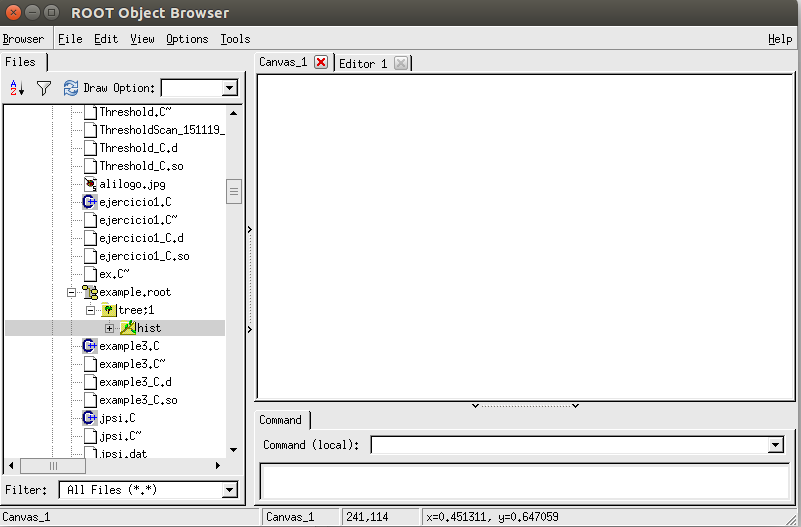
\includegraphics[scale=0.4]{browser.png}
\end{center}
\par
Regresando al archivo que gener\'o la macro, vamos a extraer los objetos usando una segunda macro.

\begin{tcolorbox} [breakable]
\begin{verbatim}
#include "TH1F.h"
#include "TH2F.h"
#include "TF1.h"
#include "TFile.h"
#include "TTree.h"
#include "TMath.h"
#include "TGraph.h"
#include "TString.h"
#include "TCanvas.h"
#include <stdio.h>
#include <fstream>

Int_t read3(Int_t entry){

TFile *arxiv = new TFile("example.root");
//sacamos el tree con su nombre.
TTree *tree = (TTree*)arxiv->Get("tree");
//Declaramos un espacio de memoria
//en donde entrara el objeto
//que recuperemos.
TH2F * hist;
//Indicamos la direccion dentro del tree
//que acabamos de recuperar y lo asociamos
//al espacio de memoria de arriba.
tree->SetBranchAddress("hist",&hist);
//Sacamos una entrada.
tree->GetEntry(entry);
//Este objeto tiene toda la informacion del objeto anterior.
hist->Draw("COLZ");

return 1;

}
\end{verbatim}
\end{tcolorbox}

\subsection{Tutoriales}

Esta gu\'ia est\'a por terminarse, as\'i que antes, dejar\'e un \'ultimo consejo. En la carpeta de instalaci\'on de Root hay una carpeta llamada tutorials. Aqu\'i hay muchas macros muy \'utiles. Tambi\'en puedes consultar otras gu\'ias en internet. Busca varias porque una sola no termina de cubrir todo lo que puedes ver en Root. Por \'ultimo, lo m\'as \'util en root, as\'i como en casi todo lo relacionado a computaci\'on, son los \textbf{foros}. Siempre que tengas una duda revisa en internet. Si en un foro encuentras a alguien llamado Ren\'e Brun, tu duda ha sido resuelta. Conf\'ia en \'el. Si tu duda no est\'a en los foros, ponla. Quiz\'a alguien m\'as adelante lo agradezca.\\
Terminaremos con una macro que difumina im\'agenes.
\begin{tcolorbox} [breakable]
\begin{verbatim}
#include "TH1F.h"
#include "TH2F.h"
#include "TF1.h"
#include "TFile.h"
#include "TTree.h"
#include "TMath.h"
#include "TGraph.h"
#include "TString.h"
#include "TCanvas.h"
#include <stdio.h>
#include <fstream>
#include "TStyle.h"
#include "TASImage.h"

void blurr(TString fName, UInt_t kN = 5)
{
   //El parametro es el nombre de la imagen + direccion.
   TASImage image(fName);
   //Obtenemos las dimensiones de la imagen
   UInt_t yPixels = image.GetHeight();
   UInt_t xPixels = image.GetWidth();
   //Sacamos el ARGB de la imagen. Esto incluye RGB + Alpha.
   UInt_t *argb   = image.GetArgbArray();

   TH2D* h = new TH2D("h","Image Histogram",xPixels,-1,1,
   yPixels,-1,1);

   for (UInt_t row=0; row<xPixels; ++row) {
      for (UInt_t col=0; col<yPixels; ++col) {
         //Colocamos el valor en cada punto.
         int index = col*xPixels+row;
         //Esto solo mide intensidad.
         //Del ARGB puedes sacar los colores tambien.
         float grey = float(argb[index]&0xff)/256;
	 //He agregado esta linea porque root
	 //No pone valores en cero con SetBinContent.
	 //En el original los puntos negros se vuelven blancos.
	 if(grey==0){grey = 0.000000001;}
	 grey = grey;
         h->SetBinContent(row+1,yPixels-col,grey);
      }
   }
   //Para que tenga algo de color.
   gStyle->SetPalette(53);


   for (UInt_t row=kN; row<xPixels-kN; ++row) {
      for (UInt_t col=kN; col<yPixels-kN; ++col) {
       int index = col*xPixels+row;
	   Float_t sum = 0;
	   for (UInt_t subrow = 0;subrow<=kN;subrow++){
		   for (UInt_t subcol=0;subcol<=kN;subcol++){
			if(subcol!=0||subrow!=0){
			sum = sum + float(argb[index+subrow+subcol*xPixels]&0xff)/256;
			sum = sum + float(argb[index-subrow+subcol*xPixels]&0xff)/256;
			if(subcol==0||subrow==0) {sum = sum + 
			float(argb[index+subrow-subcol*xPixels]&0xff)/256;}
			if(subcol==0||subrow==0) {sum = sum + 
			float(argb[index-subrow-subcol*xPixels]&0xff)/256;}
			}
		    
		   }	
		}
		Float_t original = float(argb[index]&0xff)/256;
	       if (sum!=0){
			Float_t blurry = (original + sum)/(pow(kN,2));
			h->SetBinContent(row+1,yPixels-col,blurry);	
			}
		else {h->SetBinContent(row+1,yPixels-col,original);}
      }
   }

   h->Draw("COLZ");
}
\end{verbatim}
\end{tcolorbox}

------------------------------------------------Fin------------------------------------------------

\end{document}

